\documentclass{exam}
\usepackage[utf8]{inputenc}
\usepackage{upgreek}
\usepackage[margin=1in]{geometry}
\usepackage{amsmath,amssymb}
\usepackage{multicol}
\usepackage{stmaryrd}
\usepackage{graphicx}
\usepackage{caption}
\usepackage{tikz}
\usepackage{dsfont}
\usepackage{enumitem}
\usepackage{hyperref}
\usetikzlibrary{matrix}
\newcommand\tab[1][1cm]{\hspace*{#1}}
\pagestyle{head}
\firstpageheader{}{}{}
\runningheader{\examnum}{\class}{\name}
\runningheadrule
\newcommand{\class}{Fundamentos de bases de datos}
\newcommand{\term}{Facultad de Ciencias UNAM}
\newcommand{\examnum}{Tarea 02}
\newcommand{\examdate}{28/03/2022}
\newcommand{\name}{Jurassic Team}
\begin{document}

\noindent
\begin{tabular*}{\textwidth}{l @{\extracolsep{\fill}} r @{\extracolsep{6pt}} l}
\textbf{\class} & \textbf{\term}\\
\textbf{\examnum} & \textbf{\name}\\
\textbf{\examdate}
\end{tabular*}\\
\rule[2ex]{\textwidth}{2pt}

\section*{Preguntas}
%AQUI VAN LAS PREGUNTAS
\begin{questions}
	\question \textbf{Conceptos del Modelo Entidad - Relación}
	
	\begin{enumerate}[label=\alph*.]
		\item ¿Qué es un tipo de relación? Explica las diferencias con respecto a una instancia de relación.
		
		\item ¿En qué condiciones se puede migrar un atributo de algún tipo de entidad que participa en un tipo de relación binaria y convertirse en un atributo del tipo de relación? ¿Cuál sería en el efecto?
		
		\item ¿Cuál es el significado de un tipo de relación recursiva? Proporciona un par de ejemplos de este tipo de relación.
		
		\item Responde a las siguientes cuestiones, deberás indicar si son posibles o no, justificando tu respuesta. Cuando no sea posible deberás indicar alguna recomendación al respecto: ¿Un atributo compuesto puede ser llave?, ¿Un atributo multivaluado puede ser llave?, ¿Un atributo derivado puede ser llave?, ¿Un atributo multivaluado puede ser compuesto?, ¿Un atributo multivaluado puede ser derivado?, ¿Qué implicaría la existencia de una entidad cuyos atributos sean todos derivados?
		
		\item Explica el concepto de categorías (herencia múltiple) en el modelo E-R y proporciona dos ejemplos de la vida real en donde se aplique este concepto.
	\end{enumerate}
	
	\question \textbf{Entendiendo el Modelo Entidad - Relación}
	\begin{enumerate}[label=\roman*.]
		\item A continuación, se muestran tres representaciones posibles referidas a las relaciones entre alumnos, materias y profesores. Analiza cada uno de los siguientes casos y contesta las preguntas que se presentan a continuación:
		\begin{figure}[h!]
			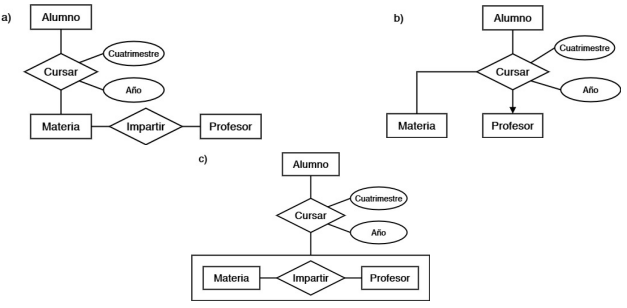
\includegraphics[scale=1]{pregunta_2_i.png}
		\centering
		\end{figure}
		\begin{itemize}
			\item ¿Los modelos presentados representan alguna realidad posible? Justifica tu respuesta
			\item ¿Los modelos mostrados representan la misma información?
			\item Qué modelo parece más apropiado para representar las siguientes situaciones:
			\begin{enumerate}[label=\arabic*.]
				\item Interesa mantener información de las materias que imparte cada profesor y en qué período.
				\item Interesa mantener información de las materias que cursa un alumno y con qué profesor. Se sabe que en un año y cuatrimestre un alumno sólo puede cursar con un profesor
			\end{enumerate}
			\item ¿Qué diferencias encuentras entre los modelos 2.i.b y 2.i.c?
		\end{itemize}
		
		\item El siguiente modelo E-R corresponde a una base de datos de compañía aseguradora de autos. Luego de unos años de funcionamiento, se han detectado una serie de deficiencias en el sistema de mantenimiento de datos y se quieren realizar las siguientes modificaciones:
		\begin{figure}[h!]
			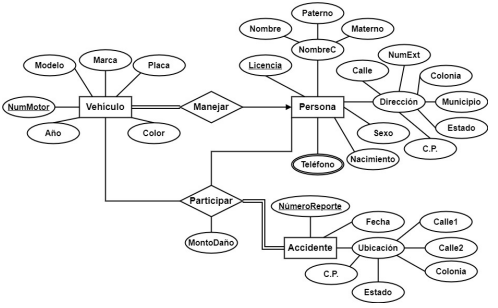
\includegraphics[scale=1]{pregunta_2_ii.png}
		\centering
		\end{figure}
		
		\begin{itemize}
			\item A la compañía le interesa llevar un registro de los agentes que atienden los siniestro, para ellos, interesan los mismos datos que las personas y un número de agente. Se debe considerar que los agentes también pueden poseer autos y potencialmente, participar en accidentes.
			\item Un vehículo puede ser manejado por más de una persona, en este caso, se requiere saber el parentesco que tiene la persona con el dueño del vehículo. Interesa poder identificar también al dueño del vehículo.
			\item Se desea almacenar información de la póliza del vehículo, la cual se identifica por un número único, tiene un tipo de seguro, cobertura, estatus y fecha de contratación. La póliza se asigna al dueño del vehículo, el cual puede tener varias pólizas. Cada vehículo pude tener una sola póliza.
		\end{itemize}				
		
	\end{enumerate}
	
	\question \textbf{Mini - mundo, planteamiento a partir del modelo Entidad - Relación}
	
	Considere un modelo de un aeropuerto con aviones, modelos de aviones, pruebas de aviones, técnicos, pilotos, aerolíneas y rutas. Desarrolla un modelo E/R para representar el siguiente modelo de negocio:
	
	\begin{itemize}
		\item Los aviones tienen un número de registro único. Cada modelo de avión se identifica con un número de modelo (por ejemplo, BJ-96) y cada uno tiene una capacidad, nombre del modelo y un peso. Cada avión es de un modelo específico y tiene asignadas las rutas que va a viajar.
		\item Se requiere mantener información de las aerolíneas que operan en el aeropuerto, para cada una de ellas se tiene un nombre, página Web y teléfonos de contacto.
		\item Los diferentes aviones que posee una aerolínea no pueden tener el mismo número de registro dentro de la aerolínea, pero dos diferentes aerolíneas podrían tener el mismo número de registro para dos aviones diferentes.
		\item Interesa almacenar la información de los pilotos de avión. Los datos que interesan son: nombre completo, número de horas de vuelo, teléfonos de contacto, la dirección, el salario y el tipo de licencia que posee (para avión comercial, avión privado o aviación ligera). Los pilotos pueden pilotar varios aviones, nunca en el mismo período.
		\item Varios técnicos trabajan en el aeropuerto y para cada uno de ellos se desea almacenar el nombre completo, sus teléfonos de contacto, la dirección y el salario. Cada técnico es experto en uno o más modelos de aviones. Su experiencia puede coincidir con la de otros técnicos.
		\item El aeropuerto tiene una serie de pruebas que se utilizan regularmente para garantizar que los aviones estén seguros. Cada prueba tiene un número único, un nombre y una puntuación máxima posible.
		\item Se requiere que el aeropuerto realice un seguimiento de cada vez que se prueba un avión determinado mediante una prueba determinada. Para cada evento de prueba, la información necesaria es la fecha, la cantidad de horas dedicadas a realizar la prueba y la puntuación que recibió el avión en la prueba.
		\item Hay rutas de aviones, cada una operando dentro de una sola ciudad. Las rutas tienen un número que es único dentro de una aerolínea, pero dos aerolíneas pueden tener rutas con el mismo número en la misma ciudad. Cada ciudad tiene un nombre único dentro de un estado, aunque puede repetirse el nombre de la ciudad en diferentes estados.
	\end{itemize}		
	
	\question \textbf{Modelo E/R}
	
	Considera el modelo Entidad/Relación que se propone a continuación, el cual representa la operación de una cadena de farmacias. Responde a las siguientes cuestiones con respecto al modelo presentado. Justifica tus respuestas.
	
	\begin{figure}[h!]
		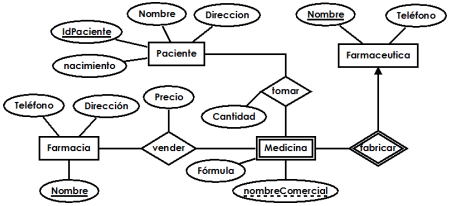
\includegraphics[scale=1]{pregunta_3.png}
		\centering
	\end{figure}
	
	\begin{enumerate}[label=\alph*.]
		\item ¿Puede una compañía farmacéutica tener múltiples números de teléfono?
		\item Si borráramos de la base de datos a la compañía farmacéutica que fabrica un medicamento, ¿qué sucede con los medicamentos que fabrica?
		\item ¿Qué ocurriría si elimináramos la farmacia que vende el medicamento? ¿Tendríamo que eliminar el medicamento también?
		\item ¿Se permite que una farmacia venda medicamentos en exclusiva? En caso que no, ¿qué se necesitaría para permitir esta característica?
	\end{enumerate}
	
\end{questions}

\noindent
\rule[2ex]{\textwidth}{2pt}
\newpage
\section*{Respuestas}
%AQUI VAN LAS RESPUESTAS
\begin{questions}
	\question \textbf{Conceptos del Modelo Entidad - Relación}
	\begin{enumerate}[label=\alph*.]
		\item Una relación es una asociación entre dos tipos de entidades, en el diagrama entidad relación se representa mediante un rombo:
		\begin{figure}[h!]
	        \centering
	        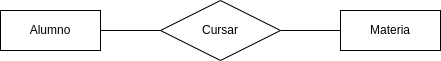
\includegraphics[width=8cm]{imgNolasco/1.png}
	    \end{figure}
		\\En ocasiones si la relación tiene varios atributos, se prefiere usar una entidad asociativa, la cual asocia a uno o más tipos de entidad y contiene los atributos peculiares de la relación:
		\begin{figure}[h!]
	        \centering
	        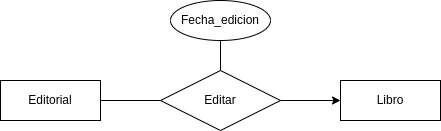
\includegraphics[width=8cm]{imgNolasco/2.png}
	    \end{figure}
	    
		\item Para responder a esta pregunta se puede pensar en la relación Alumno -- Cursar -- Materia. Al finalizar de cursar una materia un alumno obtiene una calificación para dicha materia, por lo que inicialmente se podría pensar como un atributo del tipo de entidad Materia, sin embargo una materia puede ser cursada por varios alumnos y cada uno de estos puede obtener una calificación distinta. Con esto último podemos ver que en realidad el atributo Calificación tiene sentido sólo cuando se relaciona un alumno con una materia, ahí es cuando podemos mover ese atributo a la relación.
		\begin{figure}[h!]
	        \centering
	        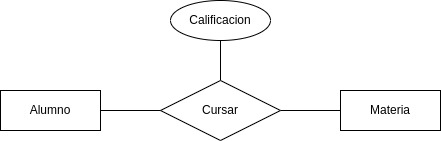
\includegraphics[width=8cm]{imgNolasco/3.png}
	    \end{figure}
	    
	    \item Una relación recursiva es aquella que relaciona a un tipo de entidad consigo misma. Esto se puede dar si entre dos tipos de entidades no hay diferencia alguna en concepto o atributos, por ejemplo, un Empleado puede ser supervisado por su Jefe directo, sin embargo el Jefe directo también es un empleado que puede ser supervisado por otro Jefe directo o no; aquí se puede usar este tipo de relación. A continuación se muestran dos ejemplos, el primero es aquel que establece que un Empleado puede supervisar a otro empleado y el segundo establece que una Persona puede tener como hijo a otra persona.
	    \begin{figure}[h!]
	        \centering
	        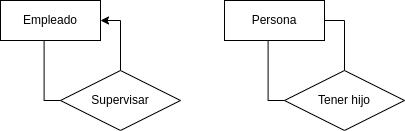
\includegraphics[width=8cm]{imgNolasco/4.png}
	    \end{figure}
	    
	    \newpage
	    \item \begin{itemize}
	    	\item Un atributo compuesto no puede ser llave por el hecho de que está compuesto por otros atributos y cada uno de ellos puede tener un dominio distinto, por lo que no podría identificar a la entidad. Se podría solucionar eligiendo otro atributo que por su naturaleza sí identifique a la entidad.
	    	\item Un atributo multivaluado tampoco puede ser llave, ya que cuenta con diferentes ocurrencias del mismo tipo de dato, por ejemplo los teléfonos de una persona, esta puede tener varios de ellos. En este caso también se debería elegir un mejor atributo que pueda identificar a la entidad.
	    	\item Un atributo no puede ser una llave porque este es calculado en cierto tiempo, por lo que de ninguna forma identifica a la entidad. Así mismo se debería buscar un atributo que identifique a la entidad.
	    	\item Un atributo multivaluado no puede ser compuesto, ya que en este atributo aparecen todas las ocurrencias y las partes de cada ocurrencia no se separan en otros atributos. Se recomienda evitar los atributos multivaluados.
	    	\item Un atributo multivaluado podría ser derivado si el cálculo da varios resultados que tienen que ser considerados. Sin embargo es difícil pensar en un caso donde el cálculo basado en ciertos atributos pueda dar varios resultados.
	    	\item La existencia de una entidad cuyos atributos son derivados implicaría que es calculada a partir de la información de otras entidades y que no podría relacionarse con otras entidades por no tener una llave primaria.
	    \end{itemize}
	    
	    \item Una categoría es una relación de superentidad/subentidad, donde hay varias superentidades. La relación siempre es
disjunta, es decir, la subclase solo puede ser una de las superentidades a la vez. En los siguientes ejemplos se puede ver que un empleado puede ser gerente o puede ser desarrollador, pero no ambos al mismo tiempo; y también que un vehículo puede ser una bicicleta o un automóvil pero no ambos.
		\begin{figure}[h!]
	        \centering
	        
\includegraphics[width=11cm]{imgNolasco/5.png}
	    \end{figure}
	    
	\end{enumerate}
	
	\question \textbf{Entendiendo el Modelo Entidad - Relación}
	
	\begin{enumerate}[label=\roman*]
	    \item 
	    \begin{itemize}
	        \item
	        \begin{enumerate}[label=\alph*]
	        \item Lo que nos dice el Diagrama es que un alumno puede tomar varias materias y éstas pueden ser tomadas por varios alumnos. Por otro lado una materia puede ser impartida por varios profesores y los profesores pueden impartir varias materias.
	        
	        Este modelo es válido si es que existen materias que sean impartidas por más de un solo profesor. Por ejemplo el alumno X inscribe Biología 1 la cual en los primeros temas es impartida por el profesor Y y en los últimos por el profesor Z.
	        
	        \item Este modelo sugiere que un profesor puede dar varias materias a varios alumnos, sin embargo, una materia que de este profesor solo la puede impartir él, y si un alumno cursa una materia con este profesor, solo puede cursar materias que imparta él.
	        
	        Este escenario puede ser posible si en una escuela imparten bloques de materias bajo un solo profesor a manera de "especializaciones" donde solo puedes elegir una especialidad aunque no tomes todas las materias de la misma. 
	        
	        \item Este modelo es parecido al de la facultad. Donde la noción de grupo está dada por la asociación entre profesor y materia. Y un alumno es libre de tomar cualquier grupo.
	        
	        \end{enumerate}
	        
	        \item Los modelos no representan la misma información tal como se describió en el anterior inciso.
	        
	        \item \begin{enumerate}
	            \item Aunque en cualquiera se puede recuperar la información, es más fácil realizar la búsqueda directamente sobre la relación cursar del \textbf{modelo C}.
	            
	            \item El \textbf{modelo B} es el único que mantiene restricción de cursar con un único profesor.
	            
	        \end{enumerate}
	        
	        \item La restricción de tomar con un solo profesor todas las materias. El modelo C permite tomar "grupos" con diferentes profesores.
	        
	    \end{itemize}
	    
	    \item Se efectúan las siguientes modificaciones:
	    
	    \begin{figure}[h!]
	        \centering
	        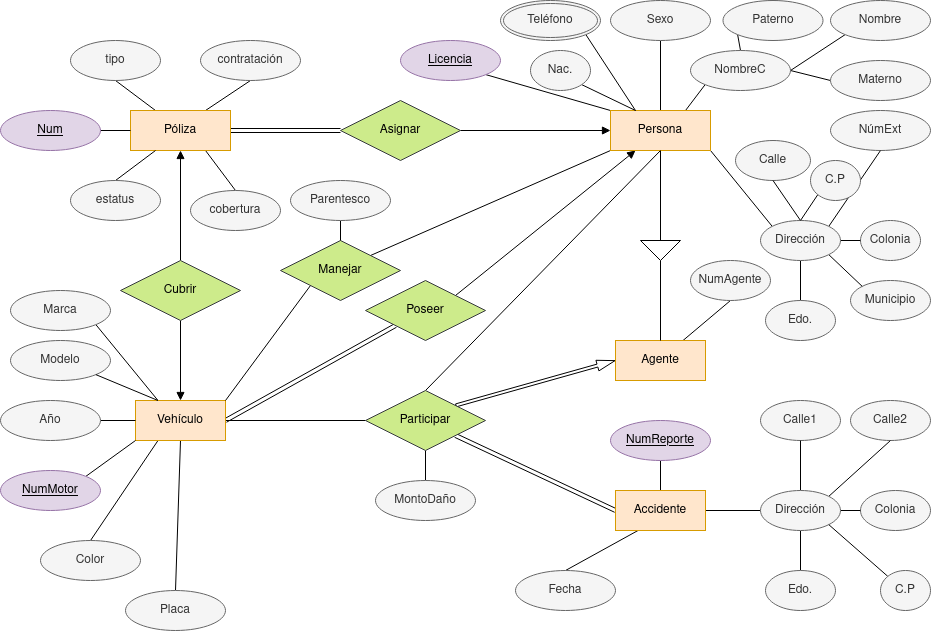
\includegraphics[width=15cm]{imgCardenas/tarea2-2-ii.drawio.png}
	    \end{figure}
	    
	    
	    \begin{itemize}
	        \item Entidades
	        \begin{itemize}
	            \item Se añade Póliza con sus respectivos atributos.
	            
	            \item Se crea la especialización Agente, la cual hereda de persona con el número de agente como único atributo.
	        \end{itemize}
	        
	        \item Relaciones.
	        \begin{itemize}
	            \item Se crea Asignar(Póliza-Persona).\\
	            Participación: Total-Parcial.\\
	            Cardinalidad: Muchos-Uno.
	            
	            \item Se crea Poseer(Vehículo-Persona).\\
	            Participación: Total-Parcial.\\
	            Cardinalidad: Muchos-Uno.
	            
	            \item Se crea Cubrir(Póliza-Vehículo).\\
	            Participación: Total-Parcial.\\
	            Cardinalidad: Uno-Uno.
	            
	            \item Se añade a la relación Participar la entidad Agente.\\
	            Participación: Total\\
	            Cardinalidad: Uno
	            
	            \item Se añade el atributo Parentezco a la relación Manejar.
	            
	        \end{itemize}
	        
	        \item Consideraciones de diseño:
	        
	        \begin{itemize}
	            \item Como un Agente es primero una persona, efectuamos especialización disyuntiva(para generar una tabla con la Licencia y Núm. de Agente como valores) y ya que es mandatorio que un Agente evalúe un incidente, la participación respecto a la relación participar es Total. Se considera además que es necesario solo un Agente para levantar el informe.
	            
	            \item Para el caso de póliza, se considera que debe tener necesariamente un beneficiario, sin embargo, como se tiene la opción de cambio de vehículo se debilita la participación. Así mismo una póliza cubre solo un vehículo y un vehículo solo puede estar asegurado por una póliza.
	            
	            \item Se crea una relación Poseer para representar al dueño de un vehículo y el atributo parentezco se agrega a Manejar.
	        \end{itemize}
	    \end{itemize}
	\end{enumerate}
	
	
	\question \textbf{Mini - mundo, planteamiento a partir del modelo Entidad - Relación}
		\begin{figure}[h!]
	        \centering
	        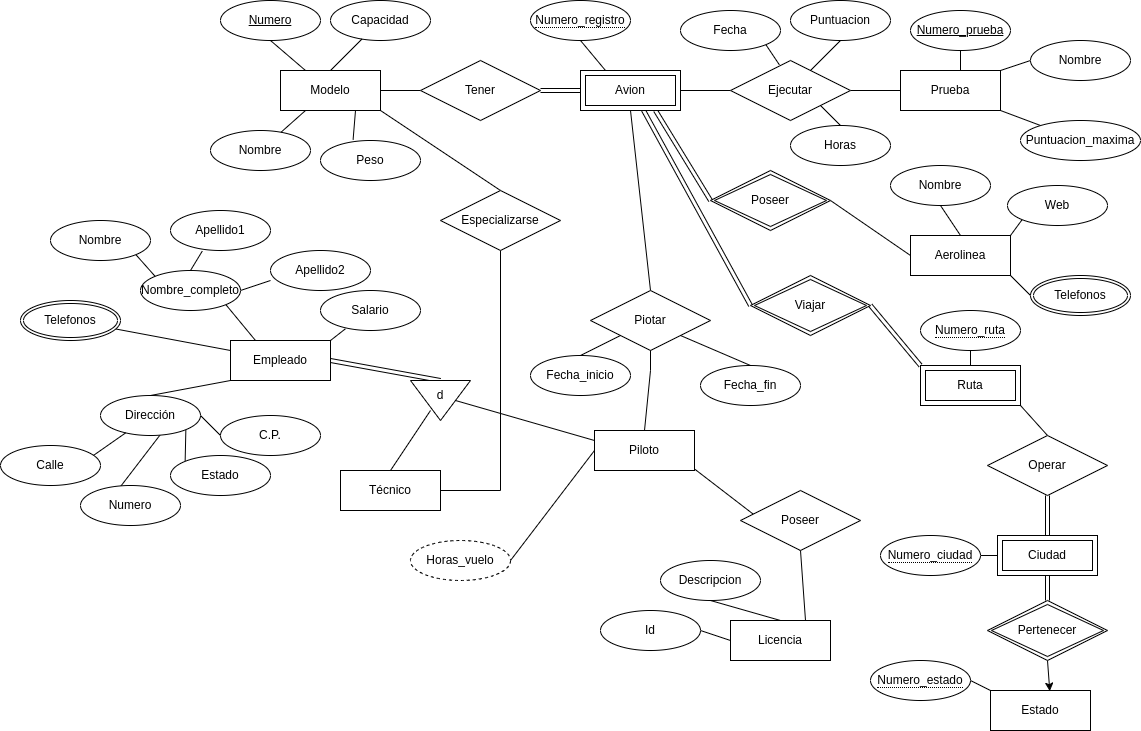
\includegraphics[width=18cm]{imgNolasco/6.png}
	    \end{figure}
	
	\question \textbf{Modelo E/R}
	
	\begin{enumerate}[label=\alph*]
	    \item Suponiendo que queremos un diseño óptimo no, dado que el atributo Teléfono no es multivaluado.
	    
	    \item Si borramos Farmacéutica estaríamos eliminando también Medicina, esto porque la segunda es entidad débil de la primera lo que hace que su llave depende de la otra.
	    
	    \item No. La participación es débil por lo tanto el medicamento puede venderse en diferentes farmacias.
	    
	    \item En este modelo no está contemplada la venta exclusiva de medicamentos. 
	    
	    Una propuesta(no muy elegante) que permita la venta exclusiva sería la siguiente: Agregar a la relación vender un atributo que indique si es de venta exclusiva o no y que al momento de definir las relaciones se indique una restricción.
	    
	    Otra propuesta sería crear una entidad(Medicina Excl) que herede de Medicina y que se relacione con farmacia mediante una relación VenderExcl(Farmacia-Medicina Excl) con cardinalidad 1:Muchos y participación parcial:parcial.
	    
	    \begin{figure}[h!]
	        \centering
	        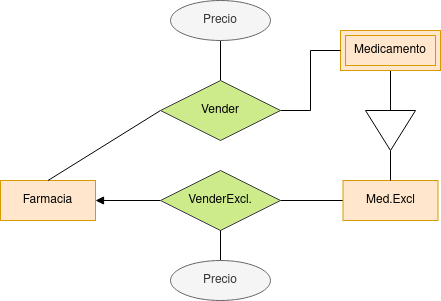
\includegraphics[width=10cm]{imgCardenas/tarea2-4-d.png}
	    \end{figure}
	\end{enumerate}
	
\end{questions}

\end{document}
